% Rows q=2,3,4,5: x in [0,1] within q^{-3} of some p/q.
% A sample line at x=1/10 meets only the q=2 row.
\begin{tikzpicture}[x=11cm,y=1cm]
  \draw[black!45] (0,0) -- (1,0);
  \draw[black!45] (0,0.85) -- (1,0.85);
  \draw[black!45] (0,1.70) -- (1,1.70);
  \draw[black!45] (0,2.55) -- (1,2.55);
  \node[left,font=\scriptsize] at (0,0) {$q=5$};
  \node[left,font=\scriptsize] at (0,0.85) {$q=4$};
  \node[left,font=\scriptsize] at (0,1.70) {$q=3$};
  \node[left,font=\scriptsize] at (0,2.55) {$q=2$};
  % q=5, radius 0.008, BurntOrange
  \fill[BurntOrange] (0,0.08) rectangle (0.008,0.36);
  \fill[BurntOrange] (0.192,0.08) rectangle (0.208,0.36);
  \fill[BurntOrange] (0.392,0.08) rectangle (0.408,0.36);
  \fill[BurntOrange] (0.592,0.08) rectangle (0.608,0.36);
  \fill[BurntOrange] (0.792,0.08) rectangle (0.808,0.36);
  \fill[BurntOrange] (0.992,0.08) rectangle (1,0.36);
  % q=4, radius 0.015625, MidnightBlue
  \fill[MidnightBlue] (0,0.93) rectangle (0.015625,1.21);
  \fill[MidnightBlue] (0.234375,0.93) rectangle (0.265625,1.21);
  \fill[MidnightBlue] (0.484375,0.93) rectangle (0.515625,1.21);
  \fill[MidnightBlue] (0.734375,0.93) rectangle (0.765625,1.21);
  \fill[MidnightBlue] (0.984375,0.93) rectangle (1,1.21);
  % q=3, radius 1/27, BurntOrange
  \fill[BurntOrange] (0,1.78) rectangle (0.037037,2.06);
  \fill[BurntOrange] (0.296296,1.78) rectangle (0.370370,2.06);
  \fill[BurntOrange] (0.629630,1.78) rectangle (0.703704,2.06);
  \fill[BurntOrange] (0.962963,1.78) rectangle (1,2.06);
  % q=2, radius 0.125, MidnightBlue
  \fill[MidnightBlue] (0,2.63) rectangle (0.125,2.91);
  \fill[MidnightBlue] (0.375,2.63) rectangle (0.625,2.91);
  \fill[MidnightBlue] (0.875,2.63) rectangle (1,2.91);
  % sample point
  \draw[BurntOrange,thick] (0.1,-0.22) -- (0.1,3.15);
  \node[BurntOrange,above,font=\scriptsize] at (0.1,3.15) {$\dfrac{1}{10}$};
  \node[below,font=\scriptsize] at (0,0) {$0$};
  \node[below,font=\scriptsize] at (1,0) {$1$};
\end{tikzpicture}
